\documentclass[12pt, twoside]{article}
\documentclass[12pt, twoside]{article}
\usepackage[letterpaper, margin=1in, headsep=0.2in]{geometry}
\setlength{\headheight}{0.6in}
%\usepackage[english]{babel}
\usepackage[utf8]{inputenc}
\usepackage{microtype}
\usepackage{amsmath}
\usepackage{amssymb}
%\usepackage{amsfonts}
\usepackage{siunitx} %units in math. eg 20\milli\meter
\usepackage{yhmath} % for arcs, overparenth command
\usepackage{tikz} %graphics
\usetikzlibrary{quotes, angles}
\usepackage{graphicx} %consider setting \graphicspath{{images/}}
\usepackage{parskip} %no paragraph indent
\usepackage{enumitem}
\usepackage{multicol}
\usepackage{venndiagram}

\usepackage{fancyhdr}
\pagestyle{fancy}
\fancyhf{}
\renewcommand{\headrulewidth}{0pt} % disable the underline of the header
\raggedbottom
\hfuzz=2mm %suppresses overfull box warnings

\usepackage{hyperref}
\usepackage{float}

\title{Algebra 2}
\author{Chris Huson}
\date{October 2023}

\fancyhead[LE]{\thepage}
\fancyhead[RO]{\thepage \\ Name: \hspace{4cm} \,\\}
\fancyhead[LO]{BECA / Huson / Algebra 2: Polynomials \\* 14 November 2023}

\begin{document}
\subsubsection*{2.10 Do Now Quiz - Find the zeros of a factored polynomial (A.APR.3)}
\begin{enumerate}[itemsep=1.5cm]
\item Write down the solutions to the following polynomial equation
\[x(x-5)(x+2)=0\]

\item Write down a polynomial function $f(x)$ with roots $x=4, -3, 7$

\item Given $f(x) = x(x+5)(x+1)(x-9)$. Select the true statements.
    \begin{enumerate}
    \item $f(5)=0$
    \item $f$ has degree 3.
    \item One of the zeros of $f$ is 9.
    \item An ordered pair satisfying the equation is $(-1,0)$
    \item $f(0)=0$
    \end{enumerate}

\item Write a recursive definition of the sequence $a_1 = 5$, $a_2 = -15$, $a_3 = 45, \ldots$

\newpage
\subsubsection*{2.10b Do Now Quiz - Find the zeros of a factored polynomial (A.APR.3)}
\vspace{-1.5cm}
\setcounter{enumi}{0}
\item Given the solutions to $f(x)=0$ are $x=0, 5, -2$. Write down a possible polynomial function $f$.

\item Write down the zeros to the following polynomial:
\[f(x) = (x-4)^2 (x+1)(x-8)\]

\item Given $f(x) = x^2(x+1)(x+5)$. Select the true statements.
    \begin{enumerate}
    \item The degree of the polynomial is odd.
    \item The $x$ intercepts of the function's graph are at $0, 1,$ and $5$.
    \item Regarding end behavior, as $x$ increases without bound in either the positive or negative direction, $y$ increases in the negative direction.
    \item An ordered pair satisfying the equation is $(-1,0)$
    \end{enumerate}

\item Write a recursive definition of the arithmetic sequence $a$. \\[0.5cm]
    \begin{tabular}{|c|c|}
    \hline
    $n$ & $a_n$ \\
    \hline
    $1$ & $-8$ \\
    $2$ & $-3$ \\
    $3$ & $2$ \\
    \hline
    \end{tabular}

\newpage
\subsubsection*{2.11 Do Now Quiz - Add, subtract, and multiply polynomials (A.APR.1)}
\vspace{-1.5cm}
\setcounter{enumi}{0}
\item Evaluate the polynomial for $x=0$:
\[f(x) = x^4-13x^2 - 23x + 17\]

\item Add $(x^4+2x^3-x^2 + 3x + 1)+(2x^4-x^3+7x^2 + 2x + 6)$

\item Simplify $(3x^4-5x^2 -9x + 10)-(x^4-4x^3+7x^2 -9x - 2)$

\item Multiply $(x^2+3) \times (2x^3-5x^2+3x+2)$ using the grid method.\\[0.5cm]
    \renewcommand{\arraystretch}{2}
    \begin{tabular}{|p{0.5cm}|p{2cm}|p{2cm}|p{2cm}|p{2cm}|}
        \hline
        & $2x^3$ & $-5x^2$ & $+3x$ & $+2$ \\
        \hline
        $x^2$ & & & & \\
        \hline
        $+3$ & & & & \\
        \hline
    \end{tabular}

\item Write a recursive definition for $a_1 = 7$, $a_2 = 1$, $a_3 = -5$, $a_4 = -11$, $\ldots$

\newpage
\subsubsection*{2.11 Do Now Quiz: Graph polynomials, identify zeros, end behavior F.IF.7c}
\vspace{-1.5cm}
\setcounter{enumi}{0}
\item Given the function $f(x)=(x-2)^2 (x+7)(x-8)$
    \begin{enumerate}
        \item Write down the zeros of the function \\[0.25cm]
        \item What is the degree of $f(x)$?
    \end{enumerate} \vspace{1cm}

\begin{multicols}{2}
    \item Write down the end behavior of the function shown at right $g(x)=x^{3}-14x+2$
    
    \columnbreak
        \begin{tikzpicture}[xscale=0.8, yscale=0.15]
            \draw [thick, ->] (-4.5,0) -- (4.5,0) node [above] {$x$};
            \draw [thick, ->] (0,-22)--(0,26) node [right] {$y$};
            \foreach \x in {-4,...,4} \draw (\x cm,3pt) -- (\x cm,-3pt) node[below] {$\x$};
            \foreach \y in {-20, -10,...,20} \draw (3pt,\y cm) -- (-3pt,\y cm) node[left] {$\y$};
            \fill (-2,0) circle[radius=0.08];
            \fill (1,0) circle[radius=0.08];
            \fill (4,0) circle[radius=0.08];
            \draw [thick, <->,smooth,samples=20,domain=-4.3:4.2] plot(\x,{(\x^3)-14*(\x)+2});
        \end{tikzpicture}
\end{multicols}

\begin{multicols}{2}
    \item Given $h(x)=x^{3}+11x^{2}+32x+28$ which is graphed below.
        \begin{enumerate}
            \item Write down the factors of the function. \\[0.5cm]
            \item Which factor has a multiplicity of 2?
        \end{enumerate} \vspace{1cm} \;
    \columnbreak
    \begin{center}
        \begin{tikzpicture}[xscale=0.7, yscale=0.15]
            \draw [thick, ->] (-8.1,0) -- (1.5,0) node [above] {$x$};
            \draw [thick, ->] (0,-13)--(0,35) node [left] {$y$};
            \foreach \x in {-8,...,-1} \draw (\x cm,13pt) -- (\x cm,-13pt) node[below] {$\x$};
            %\foreach \y in {-10,0,...,30} \draw (3pt,\y cm) -- (-3pt,\y cm) node[right] {$\y$};
            \node at (-7,0) {$\bullet$};
            \node at (-2,0) {$\bullet$};
            %\draw [thick, <->,smooth,samples=20,domain=-4.3:0.2] plot(\x,{28+(\x^3)+(11*(\x^2))+(32*\x)});
            \draw [thick, <->,smooth,samples=20,domain=-7.4:0.15] plot(\x,{(\x+7)*(\x+2)^2});
        \end{tikzpicture}
        \end{center}
\end{multicols}

\end{enumerate}
\end{document}


\begin{center}
    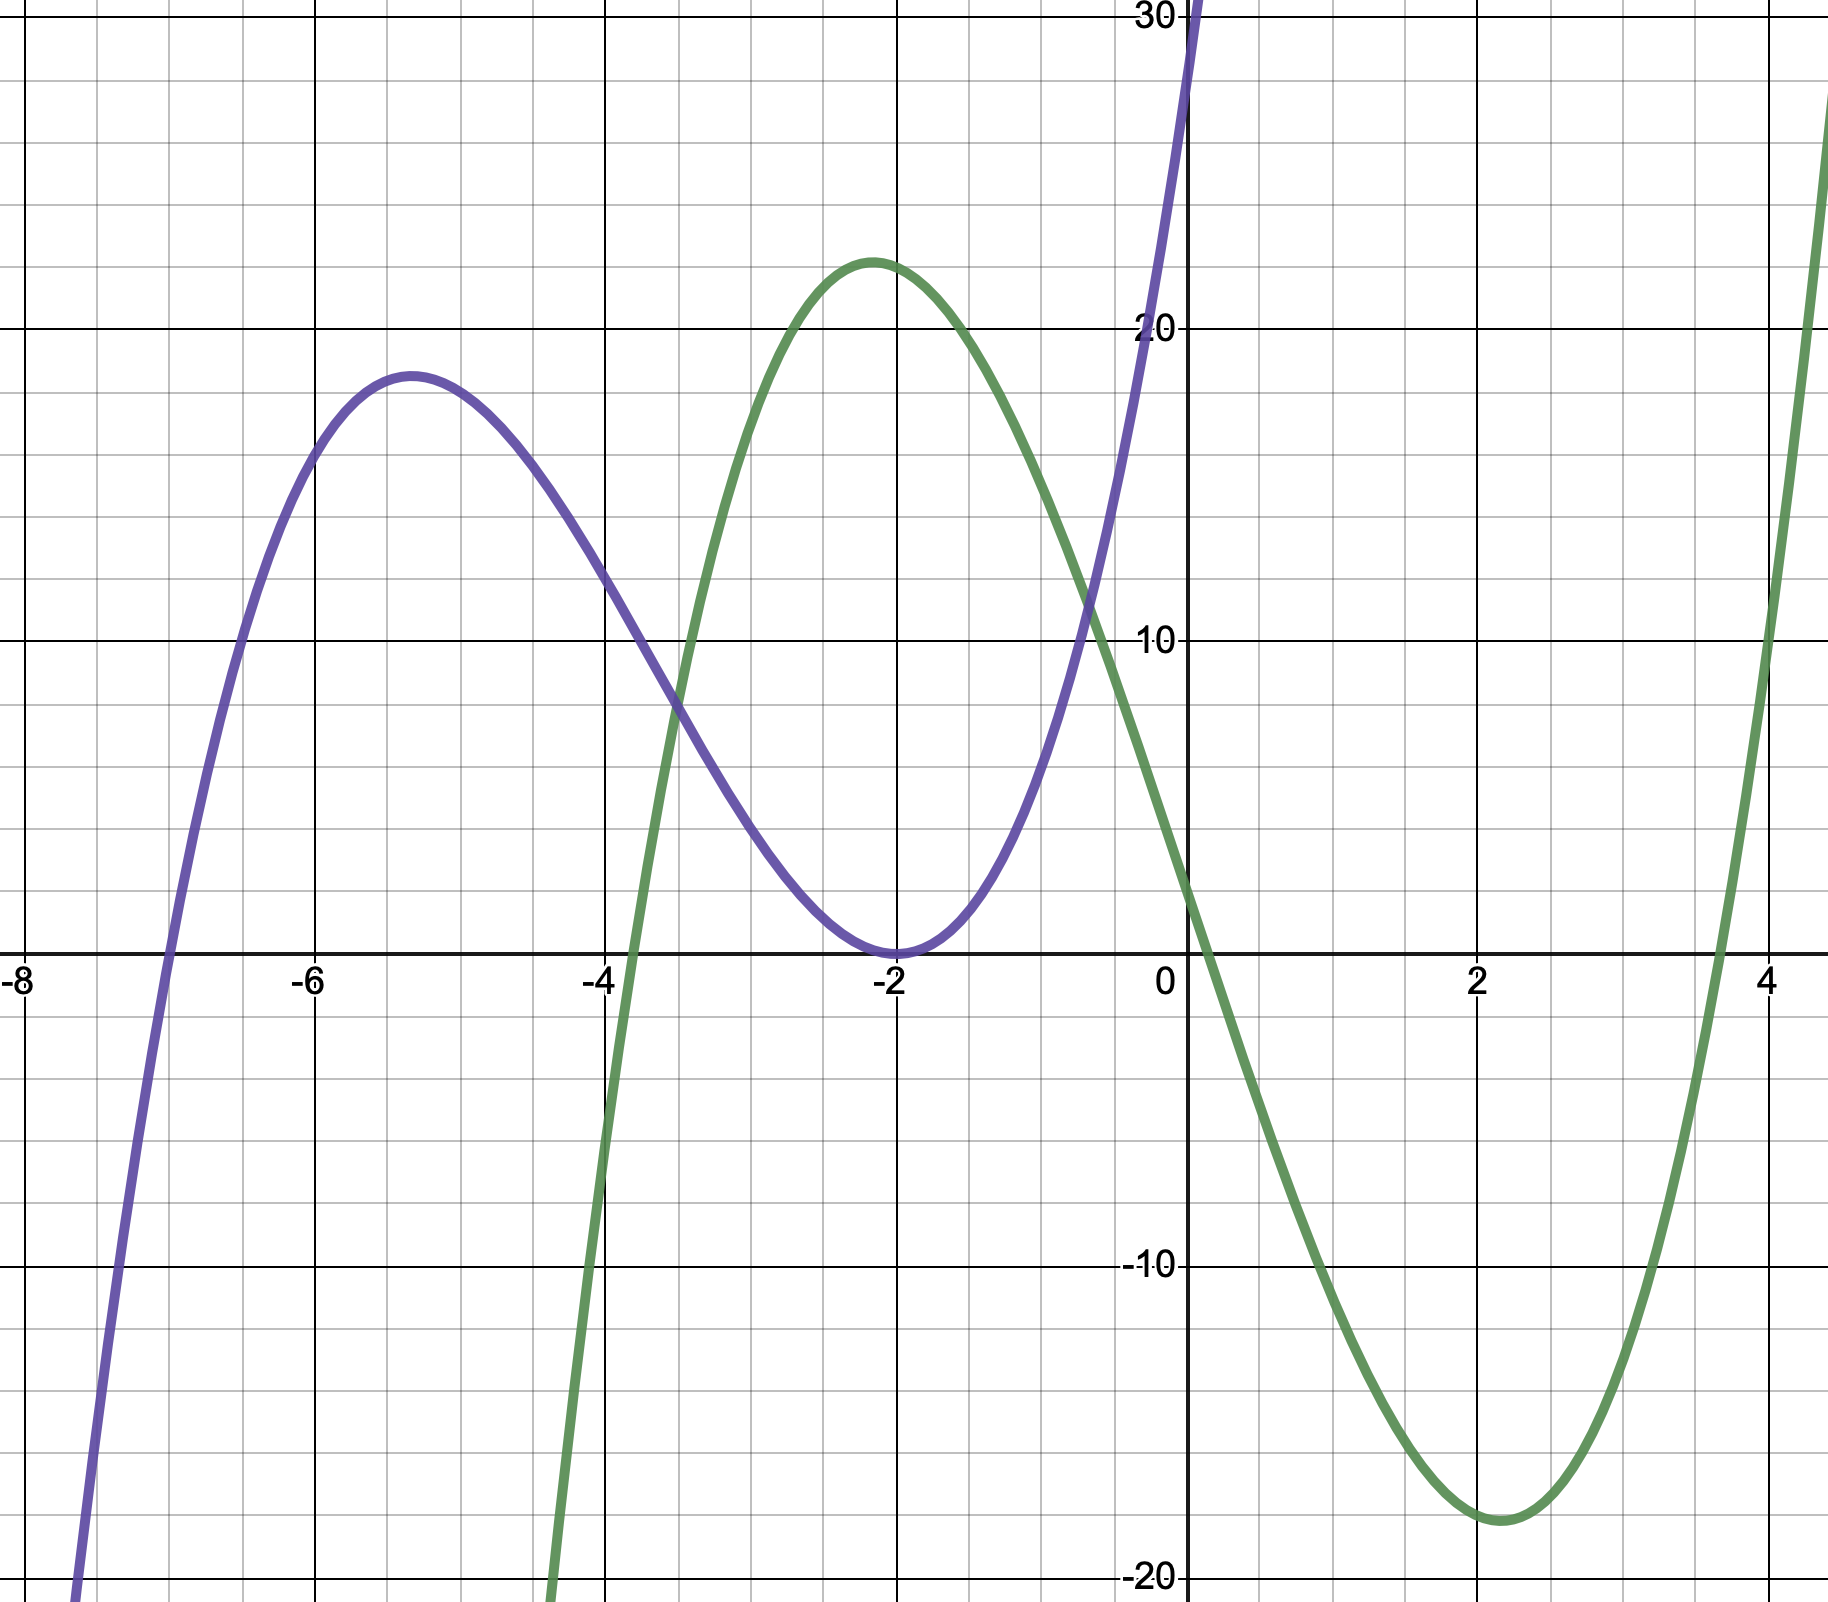
\includegraphics[width=0.6\textwidth]{../graphics/2-11DNQ-graphs.png}
\end{center}
